\documentclass{beamer}

\usepackage[frenchb]{babel}
\usepackage[T1]{fontenc}
\usepackage[utf8]{inputenc}

\usetheme{Warsaw}
\useoutertheme{infolines}

\usepackage{amsmath}
\usepackage{amssymb}
\usepackage{amsthm}
\usepackage{stmaryrd}

\usepackage[all]{xy}

%Les sous listes on des triangles
\setbeamertemplate{itemize item}[circle]
\setbeamertemplate{itemize subitem}[triangle]
%Les elements caché sont grisé
\beamertemplatetransparentcovered

\begin{document}

\title{Android - Première application}
\author{Jérémy S. Cochoy}
\institute{INRIA Paris-Saclay | jeremy.cochoy@inria.fr}
\date{Octobre 2015}


\begin{frame}
\titlepage
\end{frame}

\begin{frame}
\tableofcontents
\end{frame}

\begin{frame}
\frametitle{Quel est le but de ce cours?}

\begin{block}{Ce que vous saurez faire à la fin de cet enseignement :}

	\begin{itemize}
		\item Écrire une application Android
		\item Lire et utiliser une documentation
		\item Apprendre comment se former à une nouvelle technologie (IPhone, WindowPhone, ...)
	\end{itemize}

\end{block}

\end{frame}

\section{Pourquoi le développement mobile ?}
\begin{frame}
\frametitle{Pourquoi avons nous un smartphone?}

\begin{block}{Les smartphones ont changé notre vie de tous les jours :}

	\begin{itemize}
		\item Ecouter de la musique
		\item Regarder des vidéos
		\item Echanger du contenu multimédia via les réseaux
		\item Information en direct (bourse, journaux)
		\item Interactions sociales (snapchat, instagram, facebook et twitter...)
		\item Géolocalisation, monitoring d'activités physiques...
	\end{itemize}

\end{block}

\end{frame}
\begin{frame}
\frametitle{Pourquoi développer pour smartphones?}

\begin{block}{C'est un marché qui présente de nombreuses opportunités}

\begin{itemize}
	\item Partage d'informations (cuisine, ingénierie, journaux...)
	\item Communication entre communautés centrer autour de passion / intérêts communs
	\item Un moyen de passer le temps (jeux vidéos mobiles)
	\item Un aspect utilitaire (thermomètre, GPS, boussole...)
\end{itemize}

\end{block}

\end{frame}

\begin{frame}
\frametitle{Quelques applications...}

\begin{block}{Quelques exemples d'applications Android (certaines déjà exploitées) :}

\begin{itemize}
\item Services
    \begin{itemize}
	\item Plans de vols pour avions
	\item *Payer son restaurant via mobile
	\end{itemize}
\item Communication
	\begin{itemize}
	\item Entraide entre étudiants d'une université
	\item *Avis de ses contacts : Yes / No.
	\end{itemize}
\end{itemize}

\end{block}

\end{frame}

\begin{frame}
\frametitle{Pourquoi android ?}

\textbf{Les chiffres des ventes de mobile, fin 2015, d'après IDC.}

\begin{center}
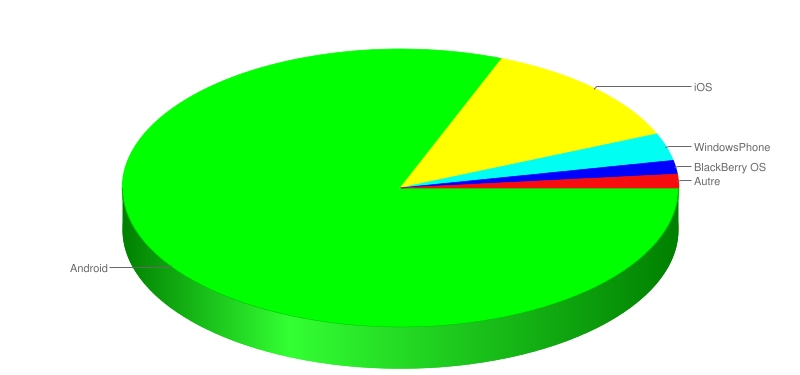
\includegraphics[scale=0.3]{marche-os-2015.png}
\end{center}

\end{frame}

\section{Genèse d'une application Android}

\begin{frame}
\frametitle{Cycle de développement}
\begin{center}
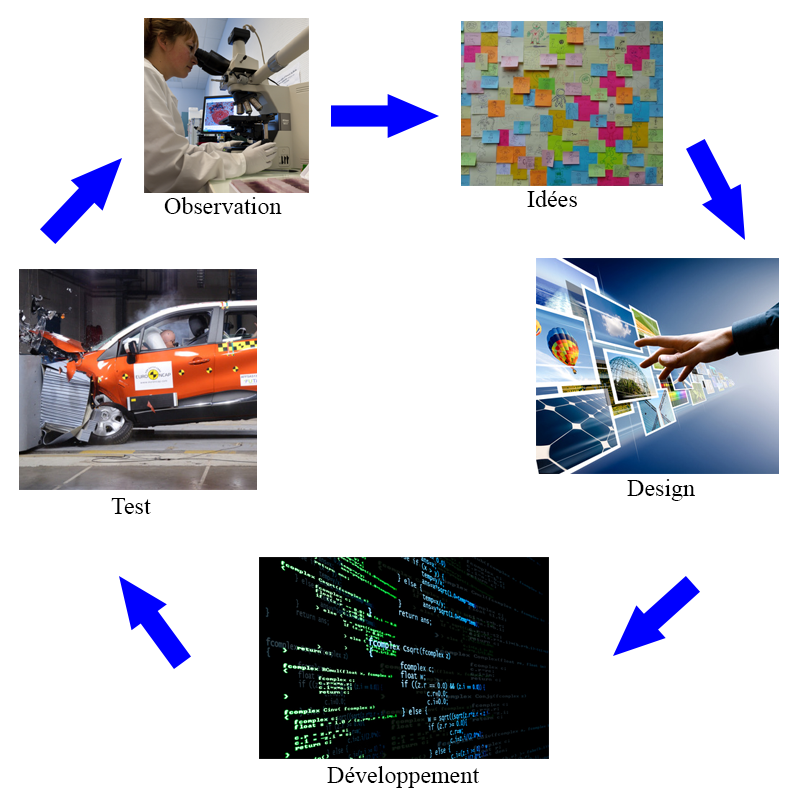
\includegraphics[scale=0.25]{cour_android_1.png}
\end{center}
\end{frame}

\begin{frame}
\frametitle{Les sources d'inspiration pour le design}

\begin{itemize}
	\item S'inspirer des solutions issues du monde réel
	\item Observer le comportement et les pratiques des gens
	\item Demander l'avis de vos amis / connaissances / inconnus
\end{itemize}

\begin{center}
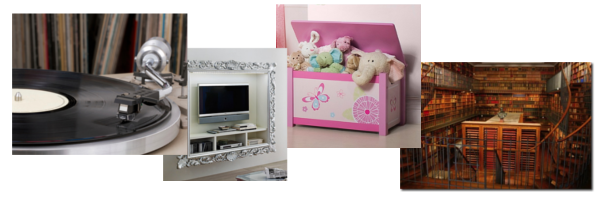
\includegraphics[scale=0.5]{design_ins.png}
\end{center}
\end{frame}

\begin{frame}
\frametitle{Le design est un processus central}

\begin{itemize}
	\item Dès le début du développement de l'application
	\item Il décrit le flot des interactions entre l'utilisateur et l'application
	\item Extrêmement important pour les petits périphériques
\end{itemize}

\begin{center}
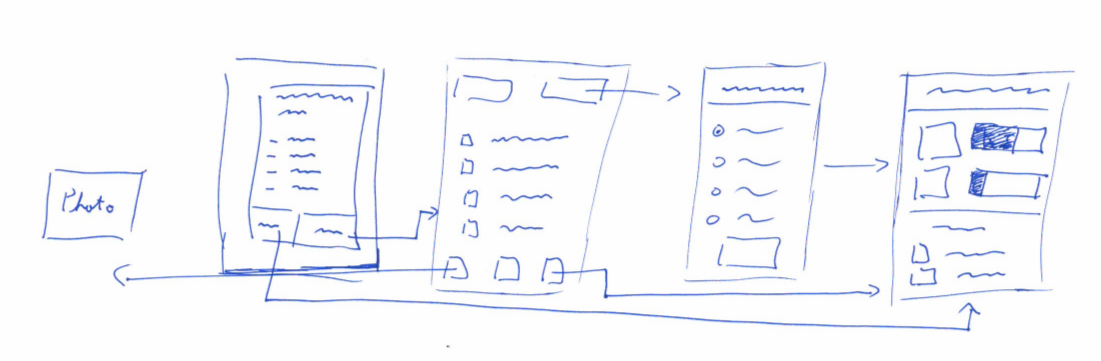
\includegraphics[scale=0.3]{design.png}
\end{center}
\end{frame}

\begin{frame}
\frametitle{Coder, tester, coder, tester ...}

\begin{block}{On doit itérer les phases de code / test}
\begin{itemize}
	\item S'assurer du bon fonctionnement par de petits tests au cours du développement
	\item Détecter les erreurs rapidement quand elles sont encore faciles à corriger
\end{itemize}
\end{block}
\begin{center}
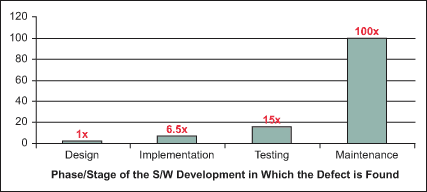
\includegraphics[scale=0.5]{defect.png}

Source : IBM Systems Sciences Institute.
\end{center}
\end{frame}

\begin{frame}
\frametitle{Ecosystème Mobile}
\begin{columns}[t]
  \begin{column}{3.5cm}
  \begin{block}{Java ME}
    \begin{enumerate}[-]
    \item Installation
    \item Pas de mise à jours
    \item Fonctionne sur diverses architectures
    \item Quelques interactions avec le téléphone
    \item Interface relativement homogène
    \end{enumerate}
  \end{block} 
  \end{column}
  
  \begin{column}{3.5cm}
  \begin{block}{Web}
    \begin{enumerate}[-]
    \item Pas d'installation
    \item Mise à jour quasi-instantané
    \item Multiplateforme : téléphones, tablettes...
    \item Interactions limitées avec le téléphone
    \item Différents rendus selon le périphérique / navigateur
    \end{enumerate}
  \end{block}   
  \end{column}

  \begin{column}{4cm}
  \begin{block}{Natif}
    \begin{enumerate}[-]
    \item Installation via Markets
    \item Mise à jour via l'OS
    \item Accès complet au téléphone
    \item Interface aux "couleurs de l'OS"
    \item Processus en arrière plan
    \item Cycle de développement / test plus complexe
    \end{enumerate}
  \end{block}
  \end{column}

\end{columns}
\end{frame}

\begin{frame}
\frametitle{Quelques domaines de recherche dans le développement mobile}

\begin{itemize}
	\item Géolocalisation
	\item Applications comportementales
	\item Applications sociales
	\item Développement personnel
	\item Compagnon devices
	\item Entreprise
\end{itemize}

\end{frame}

\begin{frame}
\frametitle{Géolocalisation}
\begin{itemize}
	\item Trouver un restaurant
	\item Déterminer le bus/métro le plus proche
	\item Tagguer des photos / événements
	\item Trouver des amis
	\item Guide touristique
	\item Réalité augmentée
\end{itemize}
\begin{center}
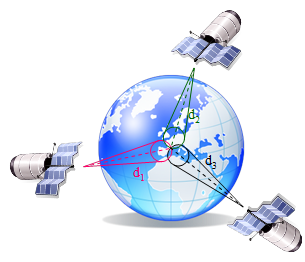
\includegraphics[scale=0.2]{geo.png}
\end{center}
\end{frame}

\begin{frame}
\frametitle{Applications comportementales}
\begin{itemize}
		\item Manger équilibré
		\item Faire des économies d'énergie
		\item Faire du sport
\end{itemize}
\begin{center}
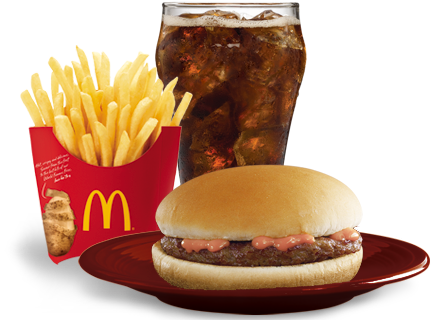
\includegraphics[scale=0.2]{burger_mcdo.png}
\end{center}
\end{frame}

\begin{frame}
\frametitle{Applications sociales}
\begin{itemize}
		\item Statuts (FB/Twitter/Line/WhatsAppp/...)
		\item Coordination (Organiser des soirées, rendez-vous, activités de groupe...)
		\item Partage de photos
		\item Partage d'emplois du temps
		\item Vendre des biens / services
\end{itemize}
\begin{center}
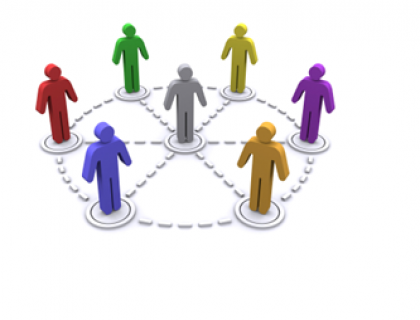
\includegraphics[scale=0.2]{social.png}
\end{center}
\end{frame}

\begin{frame}
\frametitle{Compagnon devices}

Montres, TV, Ordinateurs, Consoles, Domotique...

\begin{itemize}
		\item Afficher des informations privées
		\item Contrôle à distance
		\item Interactions hors écran
\end{itemize}

\begin{center}
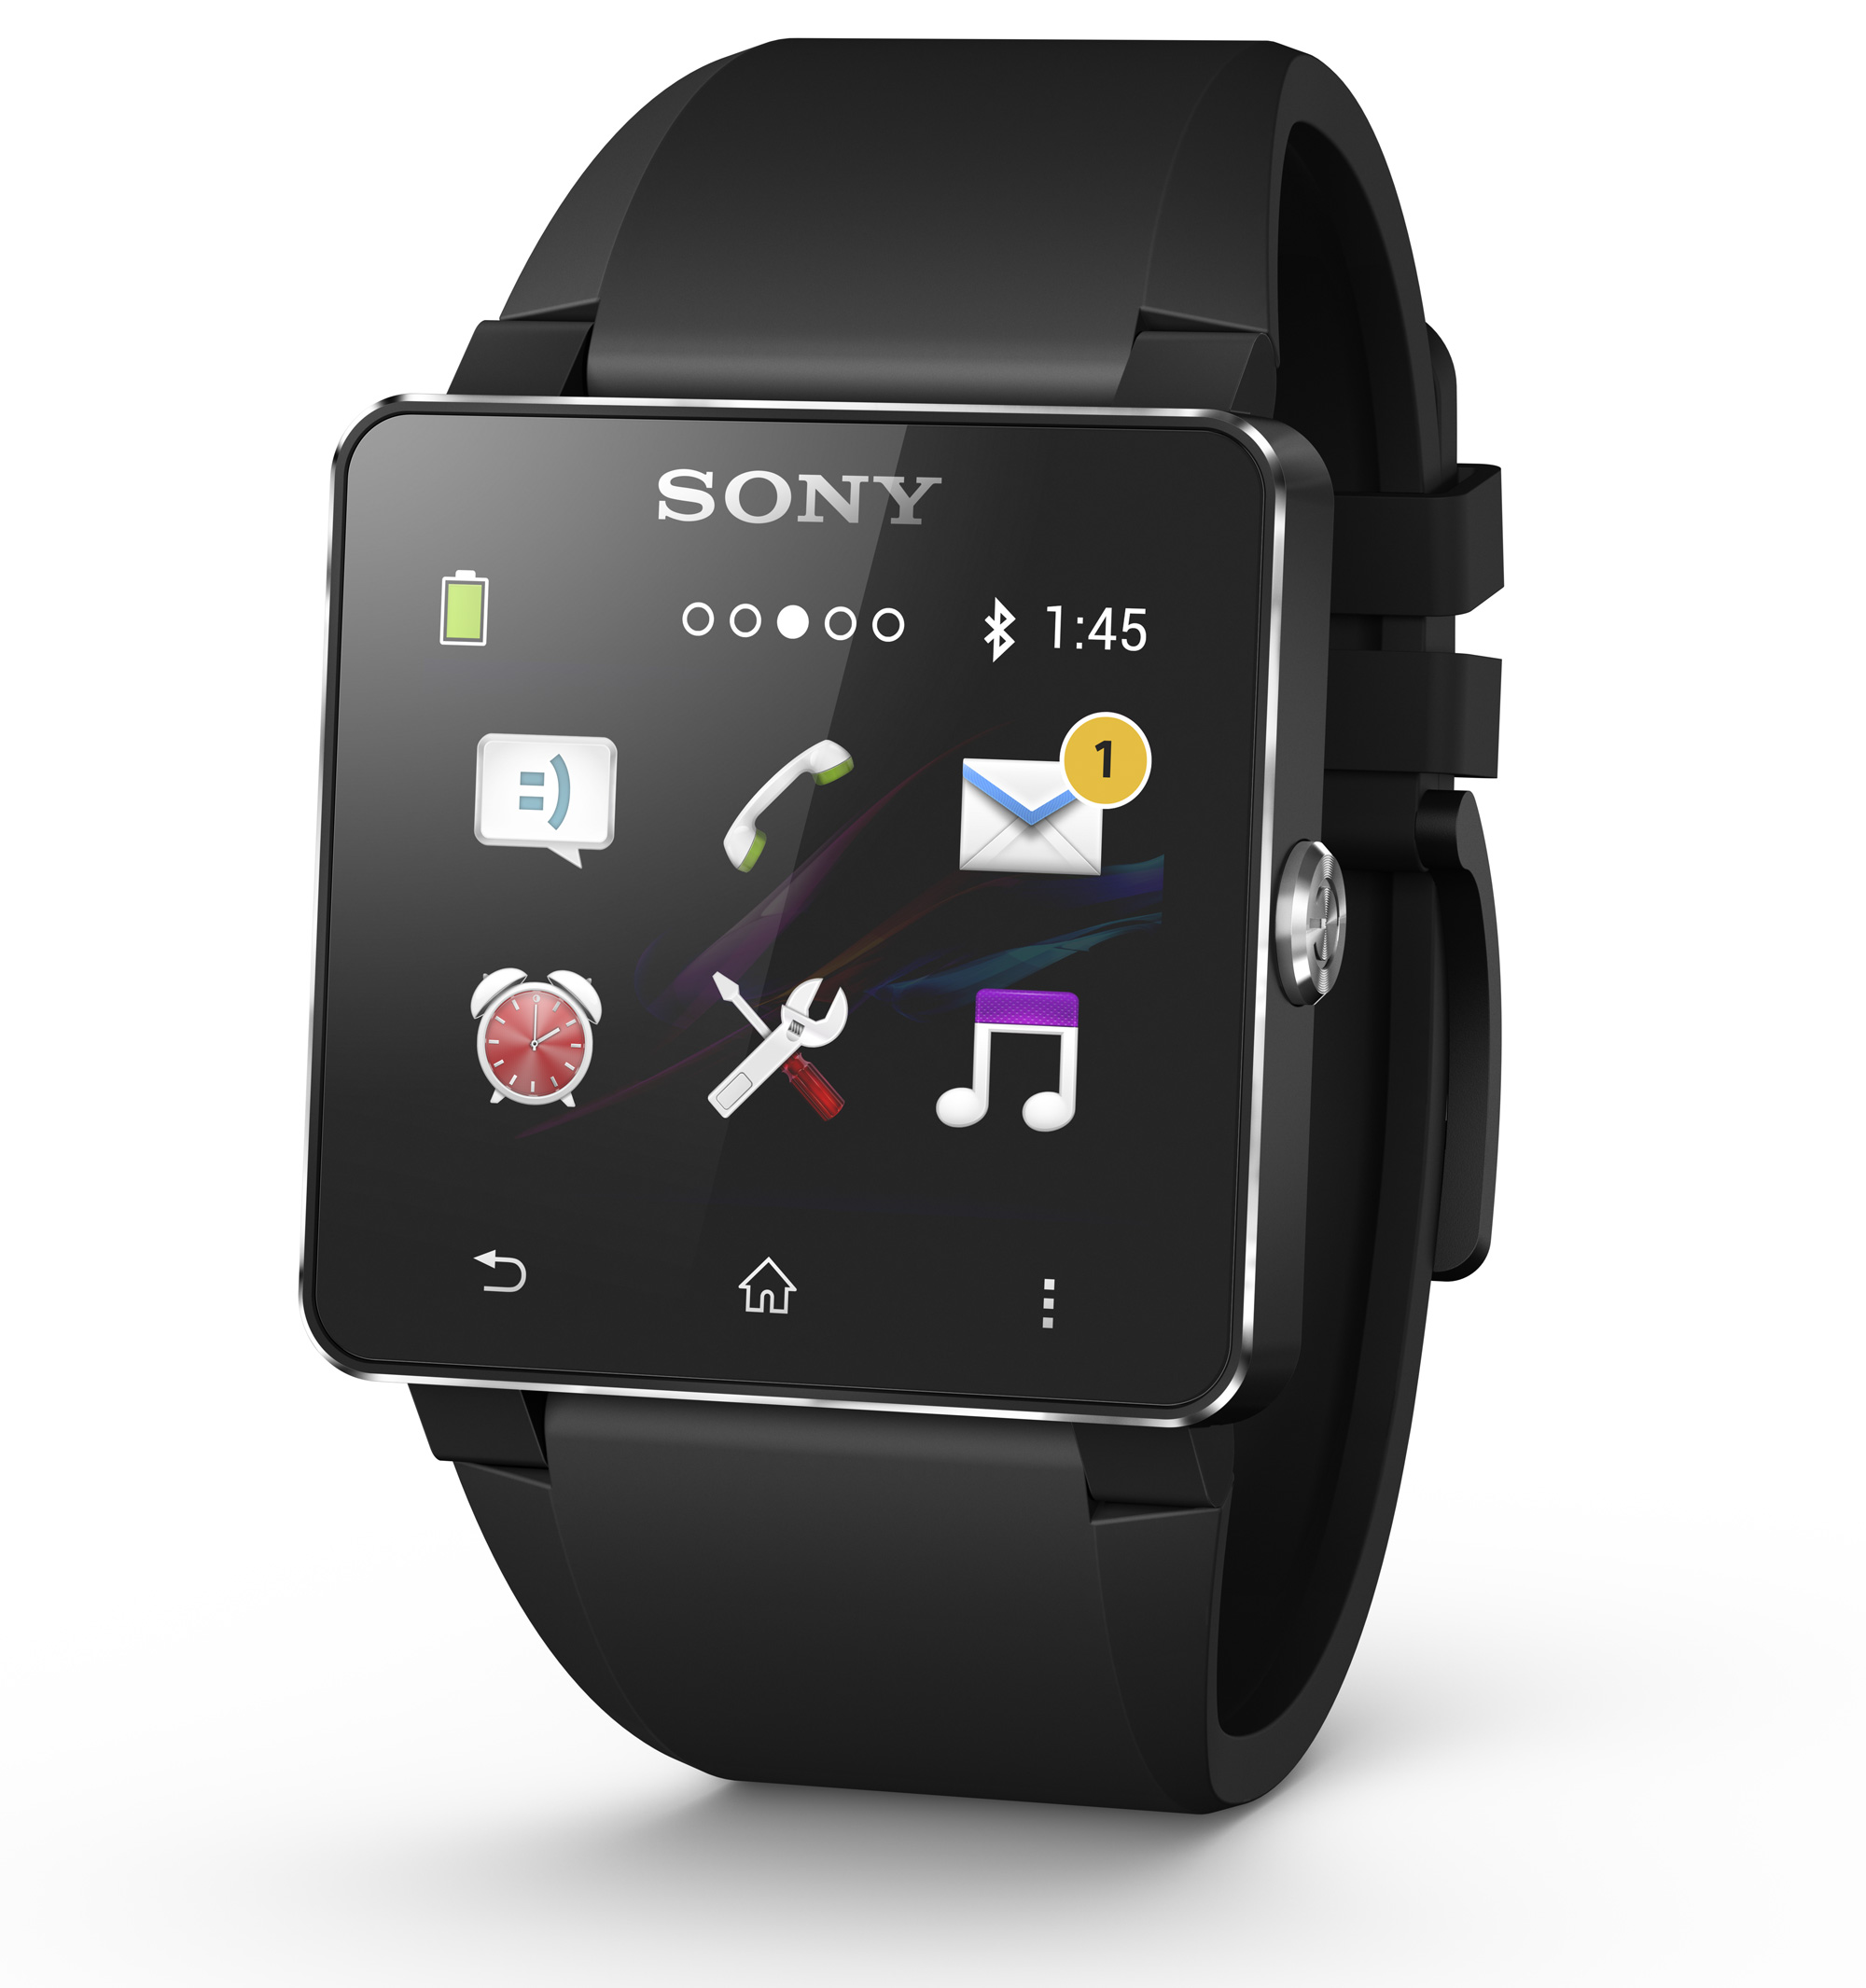
\includegraphics[scale=0.04]{montre.jpg}
\end{center}
\end{frame}

\begin{frame}
\frametitle{En entreprise}

\begin{itemize}
	\item Gestion des employer (Supermarché)
	\item Informations sur les produits en ligne / inventaire
	\item Commande dans les fast-food
\end{itemize}


\begin{center}

\includegraphics[scale=0.6]{qrcode.png}
\end{center}
\end{frame}

\begin{frame}
\begin{center}
\textbf{A votre tour. Comment utilisez vous votre téléphone?}
\end{center}
\end{frame}

\section{Trouver l'inspiration}

\begin{frame}
\frametitle{Les smartphones ne sont pas des ordinateurs}

\begin{itemize}
	\item Des interactions partout dans le monde
	\item Des interactions privées, rarement observable
	\item Des interactions brèves, étalées sur la journée.
\end{itemize}

\begin{center}
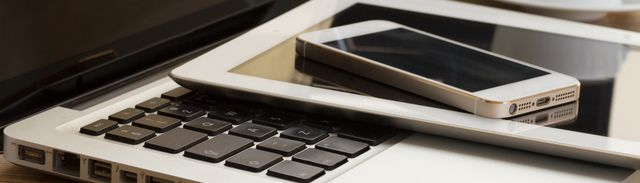
\includegraphics[scale=1]{tel-tab-lap.jpg}
\end{center}
\end{frame}

\begin{frame}
\frametitle{Sources d'inspirations}
\begin{itemize}
	\item Le design d'une application doit être basé sur la vie de tout les jours.
	\item Doit être compatible avec la façon de raisonner des gens, ce qu'ils pensent les uns des autres, et leur environnement.
	\item Quand vous sortirez, observez...
\end{itemize}
\begin{center}
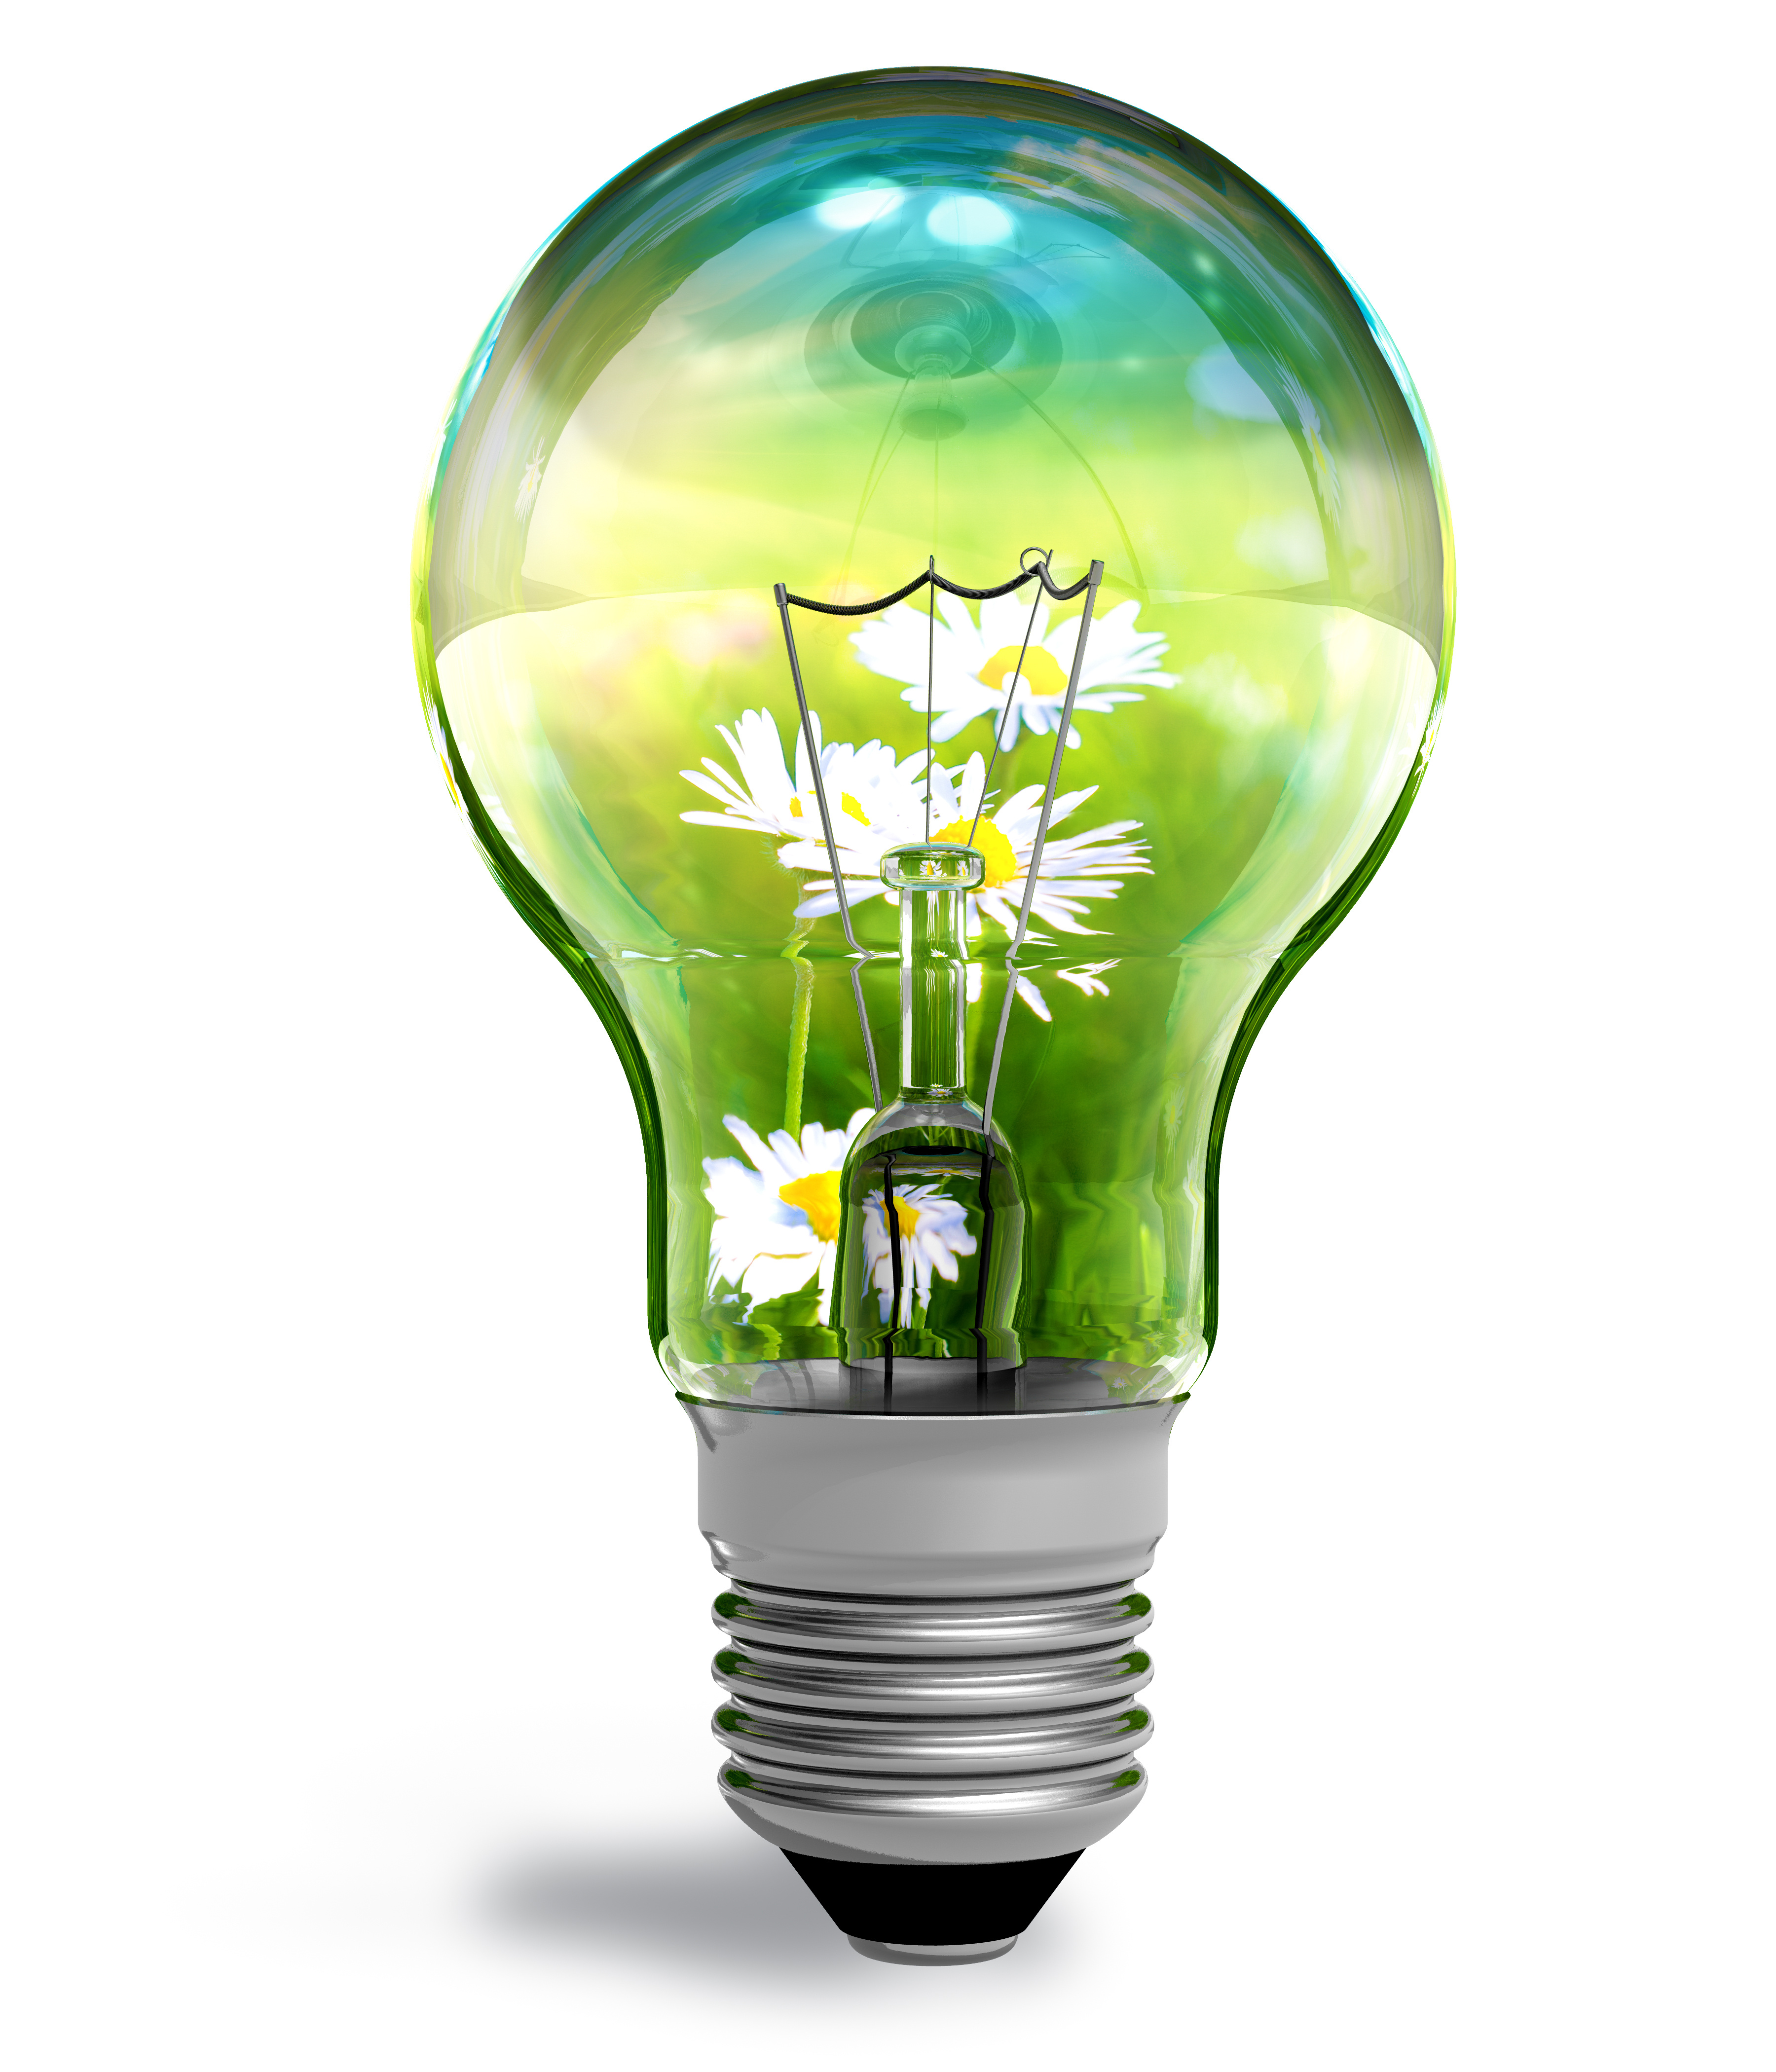
\includegraphics[scale=0.1]{idea.jpg}
\end{center}
\end{frame}

\begin{frame}
\frametitle{Processus de création}
\begin{itemize}
	\item Approfondissement d'un centre d'intérêt
	\item Dégagement de concepts et classement par priorité
	\item Implémentation d'un premier prototype (jours/semaines)
	\item Test \emph{sur le terrain} du prototype
	\item On itère les étapes 2 et 3.
	\item On convient de la forme du produit
	\item On travaille avec les markéteux, designers, vendeurs, etc. pour produire la version commerciale.
\end{itemize}
A chaque étape, le processus peut être interrompu si l'on estime avoir des doutes sur la rentabilité.
\end{frame}

\begin{frame}
\frametitle{Méthode : Observation}

\begin{itemize}
	\item Observer les intéractions des utilisateurs avec l'espace / les objets / entre eux.
	\item Observez de nombreuses personnes, déterminez les \emph{motifs}.
	\item Observez quand la durée de l'interaction et le lieu sont prédictibles.
	\item Cherchez le quoi, pas le pourquoi.
\end{itemize}

Se déplacer dans les espaces publiques / dans une épicerie.
\end{frame}

\begin{frame}
\frametitle{Méthode : Faite un tour chez un ami}
\begin{itemize}
	\item Visitez une maison / appartement, ou un bureau, et repérez les lieux d’Interactions.
	\item Bien pour observer les taches qui dépendent du contexte / se base sur des objets physiques.
\end{itemize}

Permet par exemple d'observer le comportement des utilisateurs vis à vis de la musique (CDs).
\end{frame}

\begin{frame}
\frametitle{Méthode : Journal de bord}
\begin{itemize}
	\item Tenir un journal (papier, notes vocales, etc.) quand ils effectuent des actions en rapport avec le domaine étudié.
	\item Essayez de saisir l'action sur le vif, plutôt qu'un souvenir ; plus fiable.
\end{itemize}
\end{frame}

\begin{frame}
\frametitle{Méthode : Interviews}

\begin{itemize}
	\item Pour compléter les observations directes
	\item Doit se concentrer sur la compréhension des pratiques.
	\item PAS de concept futur "est-ce que vous aimeriez, voudriez, ..." etc.
	\item Questions structurées qui s’enchaînent par ordre croissant d’intérêt.
\end{itemize}
\end{frame}

\begin{frame}
\frametitle{Ce qu'il faut rechercher :}
\begin{itemize}
	\item Qu'est-ce que les gens aiment, quelles parties d'une tache les font sourire?
	\item Quand deviennent-ils irrités, frustrés?
	\item Qu'est-ce qui est pour eux facile / difficile à faire?
\end{itemize}
\end{frame}

\begin{frame}
\frametitle{Comment poser des questions ?}
\begin{itemize}
	\item \textbf{Ne pas demander} : qu'as-tu l'habitude de faire, comment tu utilises / aime une application / fonctionnalité, ce que tu ferais dans le cas...
	\item \textbf{Demander} : La dernière fois, la fois d'avant...
	\item Posez les questions que vous avez après avoir observer quelqu'un, MAIS attendez qu'il ai terminé.
\end{itemize}
\begin{center}

\includegraphics[scale=0.5]{question.jpg}
\end{center}
\end{frame}

\begin{frame}
\frametitle{Observation semi-structuré}
\begin{itemize}
	\item But : Comprendre un domaine - Matière pour s'inspirer
	\item Processus : Quelques questions sur le domaine. Observer les gens dans leurs activités, leur poser des questions pour mieux comprendre.
	\item Écrire les citations / observations sur des post-it.
	\item Essayez d'en avoir $\sim$50.
\end{itemize}

\pause

\begin{exampleblock}{Exemple de citation}
Mon radio-réveille me réveille chaque matin. Je l’éteins et j'allume ma chaîne stéréo parce que le son est meilleur...
\end{exampleblock}

\begin{exampleblock}{Exemple d'observation}
Une pile de CDs posés sur le sol, sans boite ou rangement.
\end{exampleblock}

\end{frame}

\section{L'analyse des données}

\begin{frame}
\frametitle{Diagrammes de flux}
\begin{itemize}
	\item Développé en \emph{Contextual Dessign} par Beyer \& Holtzblatt
	\item Modélise comment les objets / informations / personnes inter-réagissent.
	\item Aide à saisir les goulots d'étranglement dans les interactions.
\end{itemize}
\end{frame}

\begin{frame}
\begin{center}
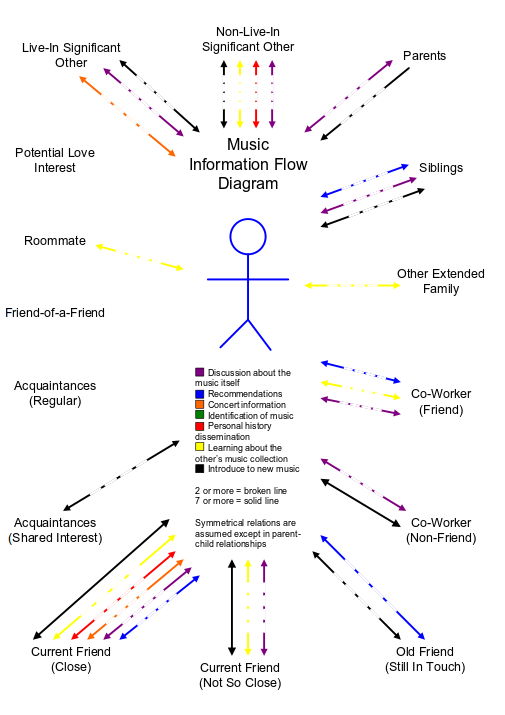
\includegraphics[scale=0.35]{flow_diag.png}
\end{center}
\end{frame}


\begin{frame}
\frametitle{Diagrammes d'affinité}
\begin{itemize}
	\item Organise les grandes quantités d'informations qualitative en thèmes.
	\item Permet de générer des bases d'explications à des phénomènes complexes.
	\item Facilite le brainstorming.
	
	\item \textbf{Mais : } ne permet pas de tester une hypothèse, de valider / rejeter une théorie.
\end{itemize}
\end{frame}

\begin{frame}
\begin{center}
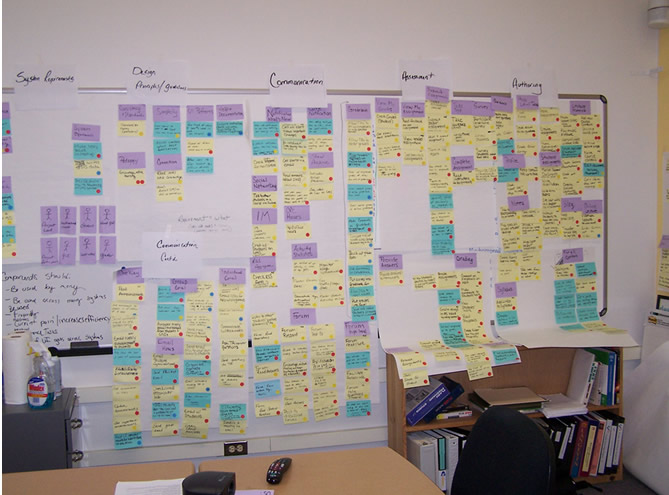
\includegraphics[scale=0.35]{afinity_diag.jpg}
\end{center}
\end{frame}

\begin{frame}
\begin{center}
\textbf{Imaginez VOTRE application Android.}
\end{center}

\begin{center}
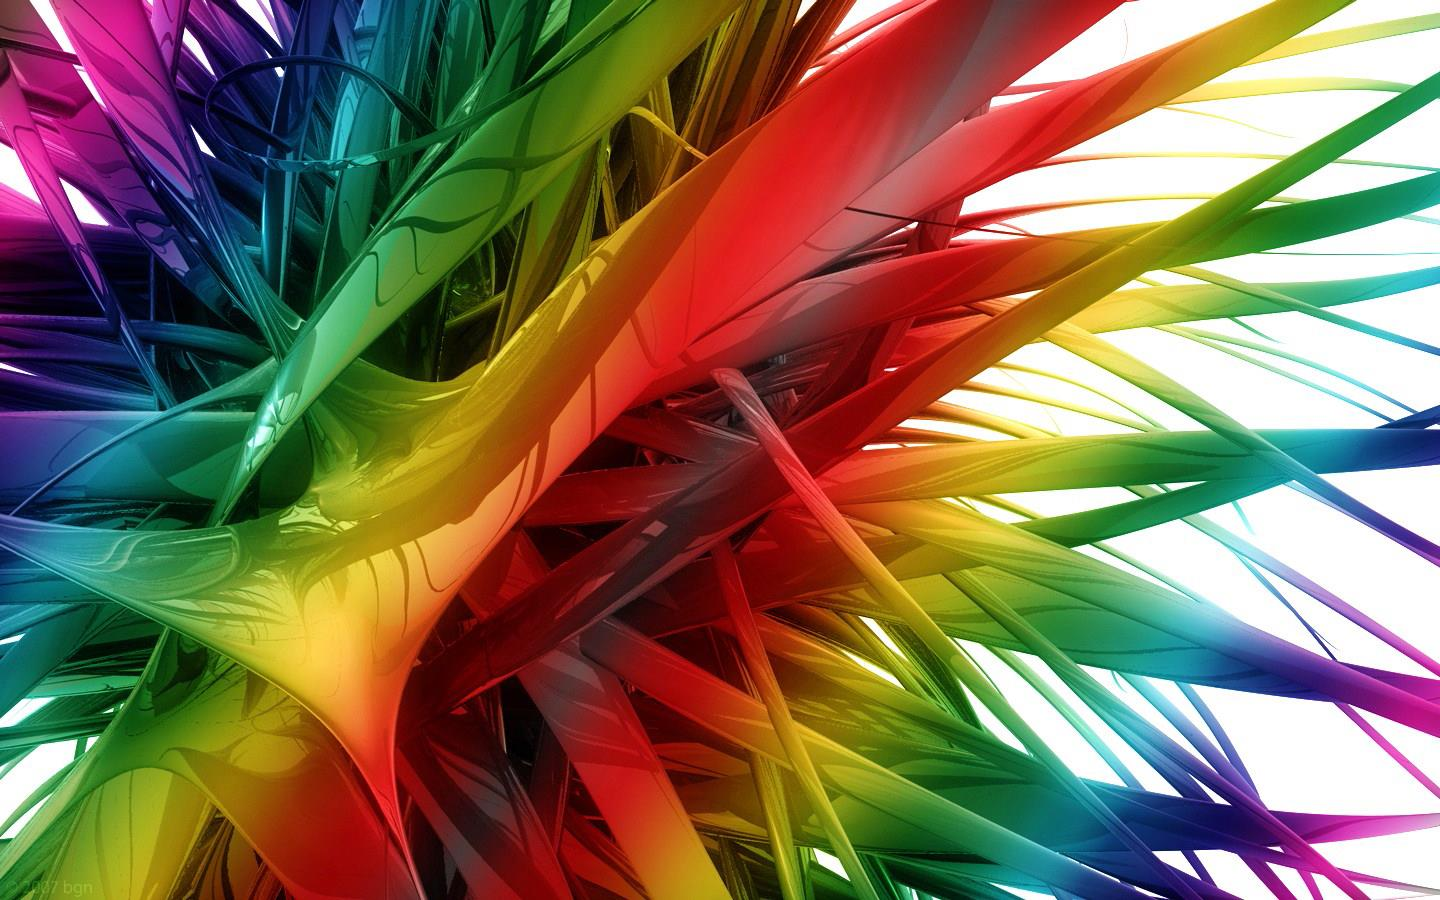
\includegraphics[scale=0.2]{couleurs.jpg}

\end{center}
\end{frame}

\section{Le cours}

\begin{frame}
\frametitle{Évaluation du cours :}

\begin{itemize}
	\item Un contrôle continu (Tous les TDs seront à rendre et notés)
	\item Un projet en groupe de 2 à 4
	\item Un examen final
\end{itemize}
\end{frame}

\begin{frame}
\frametitle{Homework}

\begin{center}
\textbf{Installez Android studio.}
\end{center}

\end{frame}

\begin{frame}
\frametitle{Compilez un projet de test}
\begin{center}
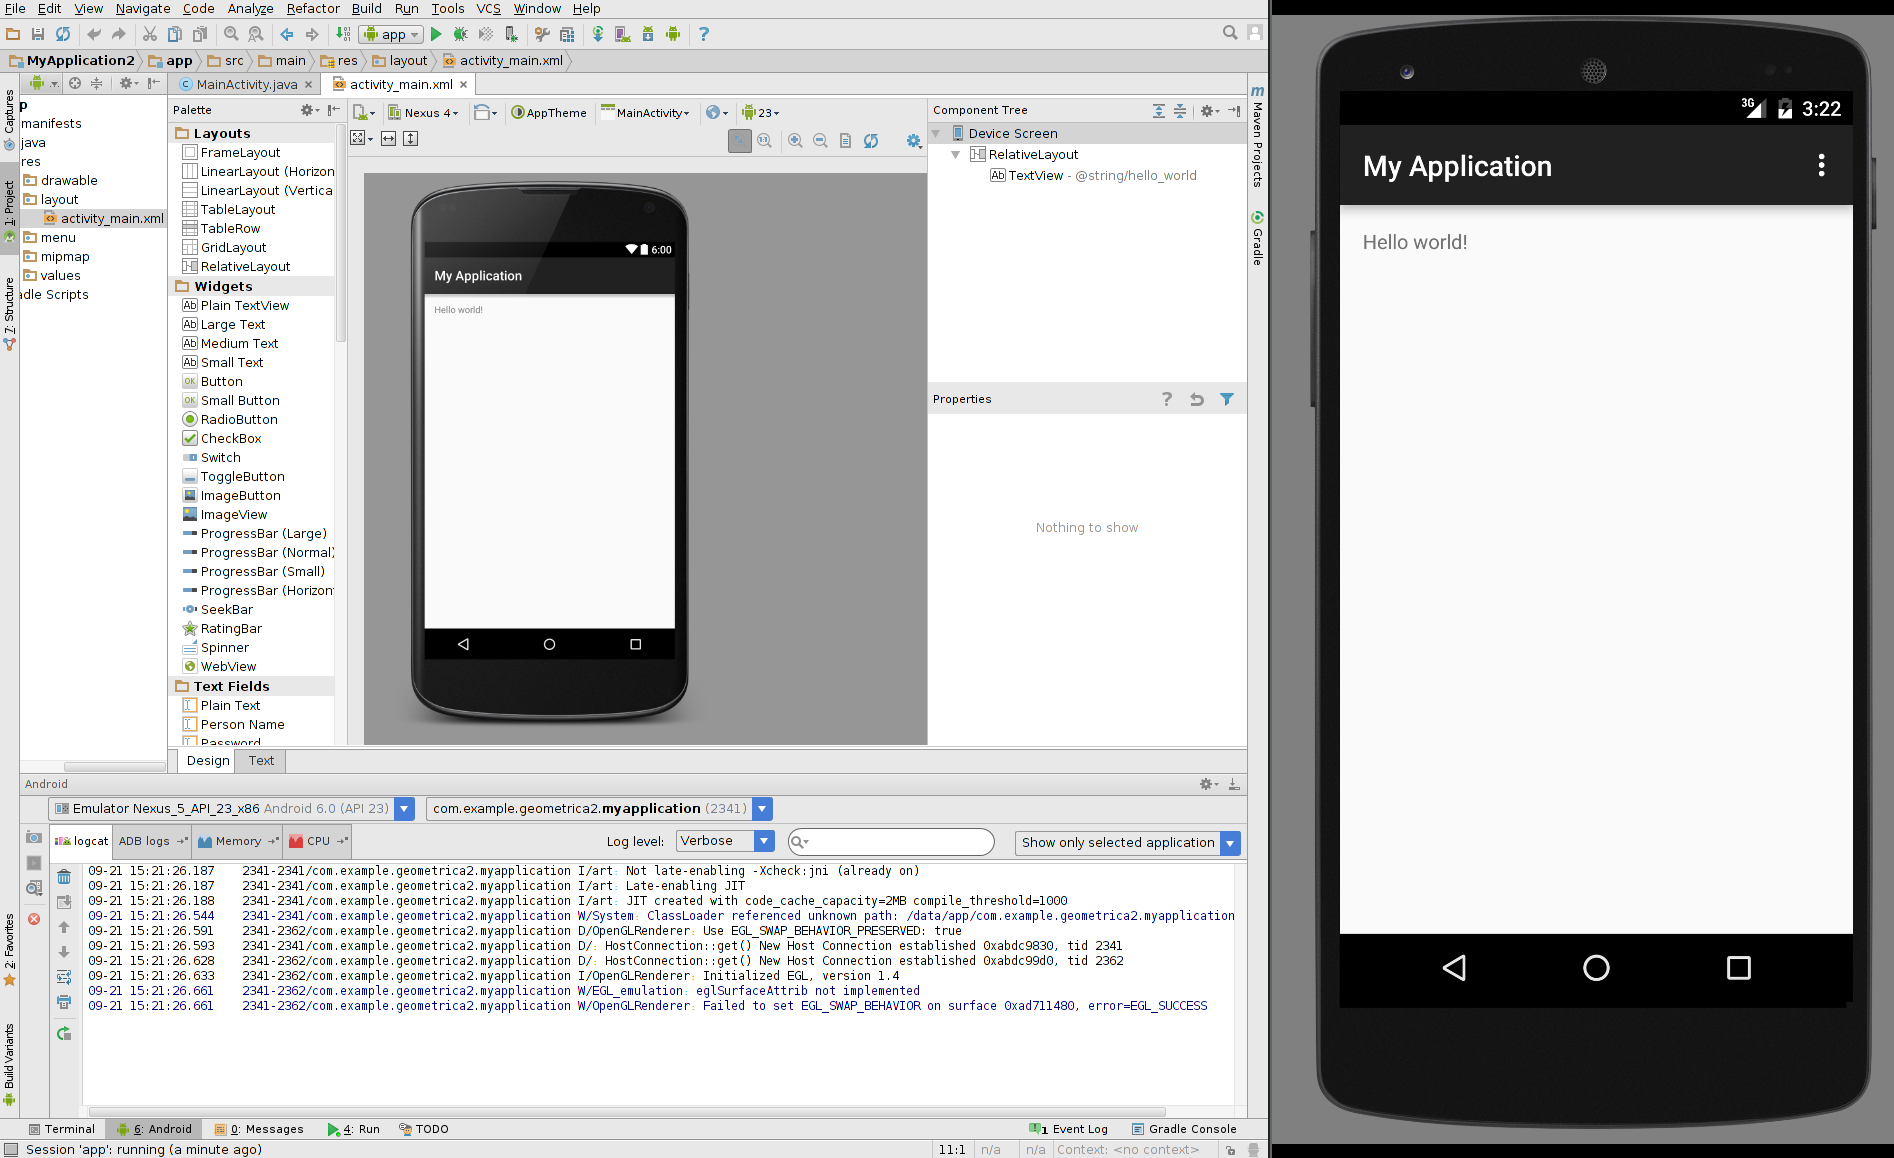
\includegraphics[scale=0.18]{android_test.png}
\end{center}
\end{frame}


\begin{frame}
Vous n'avez jamais fait de java? Entraînez vous sur CodingGame.

\begin{center}
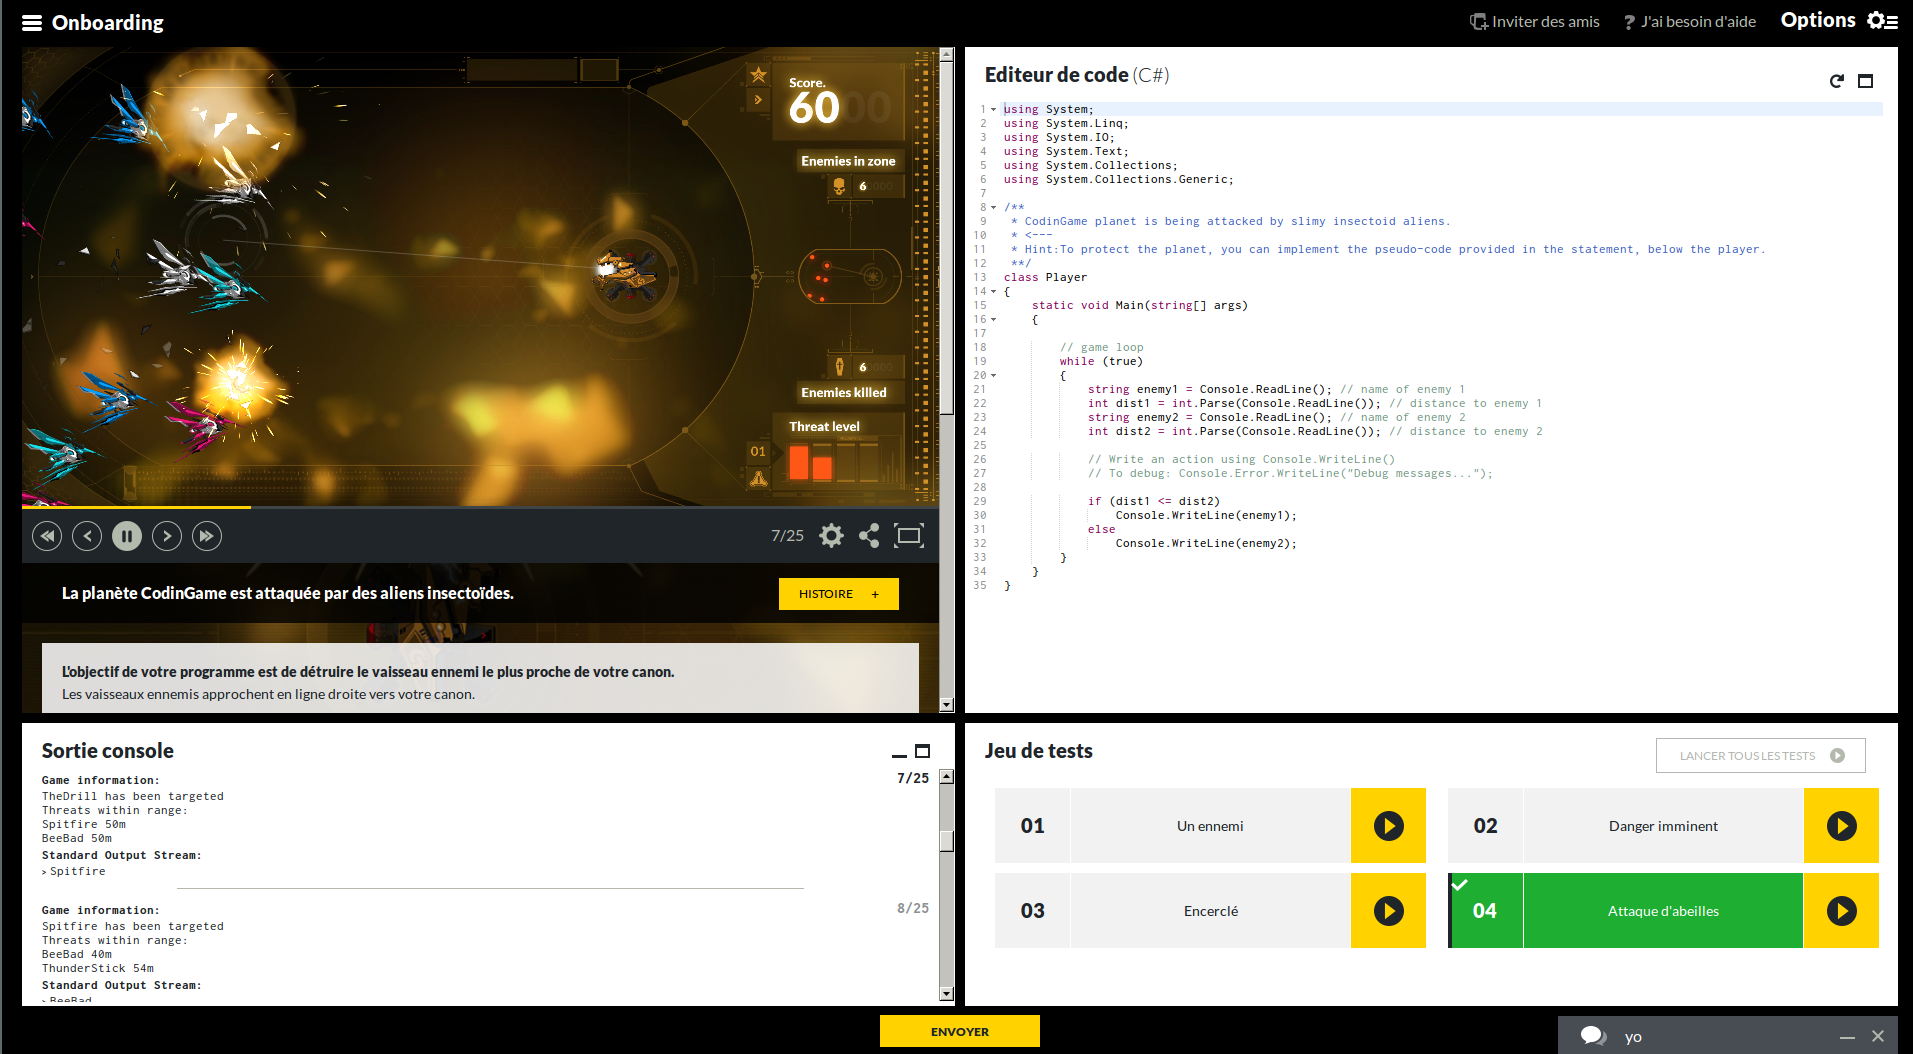
\includegraphics[scale=0.18]{codinggame.png}
\end{center}
\end{frame}


\begin{frame}
\begin{center}
Pour me contacter : jeremy.cochoy@u-psud.fr, merci et à bientôt.

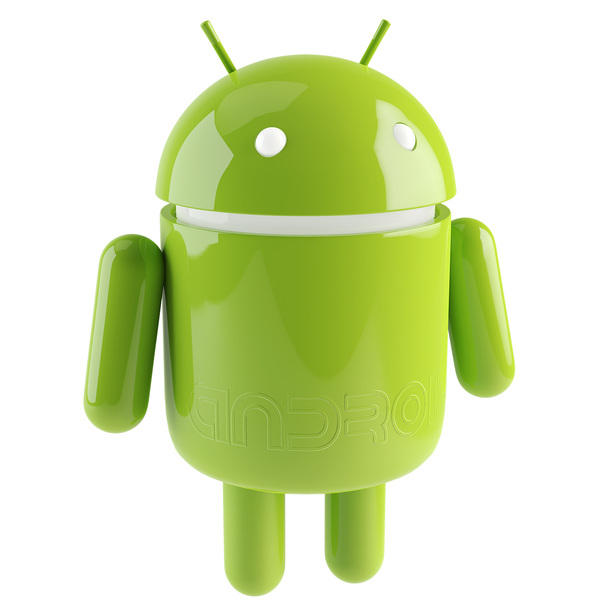
\includegraphics[scale=0.18]{android.jpg}
\end{center}
\end{frame}
\end{document}
